\section{Application} 
\label{sec:app} 
 
 
The implemented android application is responsible for communication with both the location service, already presented in Section \ref{sec:LocService}, and the maps service. 
 
 
When a user notifies the application that he wishes to start the system, the app starts a periodic operation that provides a location at the end of each iteration. At the beginning of each operation, the app requests the location service for a location. The expected answer contains a geographical location as well as additional  textual information. The data is then forwarded to the maps service. This action is the fourth and last from Figure \ref{fig:MockProvider}. 
 
 
The maps service is implemented using the Google Maps Android API. Through the usage of Google Maps, it was possible to reduce the load on the application, since there was no need implement the maps server component. Since the indoor maps of the testing environment were already available, there was no need to upload addition maps onto google maps. Having passed the entire maps server component onto the already existent service, the complexity of the system was reduced. By making this development choice, the system as a whole became closer to the desired generic approach while making possible for seamless transition between indoor/outdoor maps. The only imposed restriction is related to the addiction of new indoor maps onto the google maps, which while possible and well documented, is dependent on a third party. As previously described on Chapter \ref{cap:architecture}, upon deciding to use the google maps service as the maps server, the location description present in the location server had to be adjusted accordingly. The position description of each \ac{BLE} enabled device contained in the database were updated, so that it would be compatible with the description type used by Google maps. This change involved describing each beacon by its latitude, longitude and floor level. 
 
 
The Fourth step occurs when the application receives a location from the request made onto the location provider. With the device's location known, a marker is placed on the map with the obtain coordinates (longitude, latitude), the camera is centralised on the position while displaying the indoor level map. The menu visible on Figure ~\ref{fig:AppMenu} is updated with the information that is bundled with the received location. In order to show the correct level on a multi level building, the "floor" information present in the menu is used. The Google API is capable of providing a list of the levels of the building that is currently being focused by the map's camera. Since the location's associated floor is know, the floor can be selected from the list and the view updated. 
 
 
The pop-up menu was implemented to demonstrate the capacity of providing additional information associated with each location. While the current implementation displays the location's geo-location taxonomy, the architecture is capable of support other types of additional information, such as hyperlink or information on nearby events.   
 
 
The final state of the implemented system can be visualised in Figure ~\ref{fig:AppFocus} and Figure ~\ref{fig:AppMenu}. The first figure displays the applications main screen, where the google maps view is located. In this example: 
\begin{itemize} 
\item The user's location inside the building is represented by the red marker; 
\item The building where the user is located is focused. Upon focusing on a building, google maps provides a level selector. Through it, it's possible to select the building floor that is to be displayed; 
\item The building floor where the user is located is selected. This action updates the view with the selected floor and highlights it (floor 0) on the provided menu. 
\end{itemize} 
Figure \ref{fig:AppMenu} displays the menu containing the geo-location taxonomy. 
 
 
\begin{figure} 
\centering 
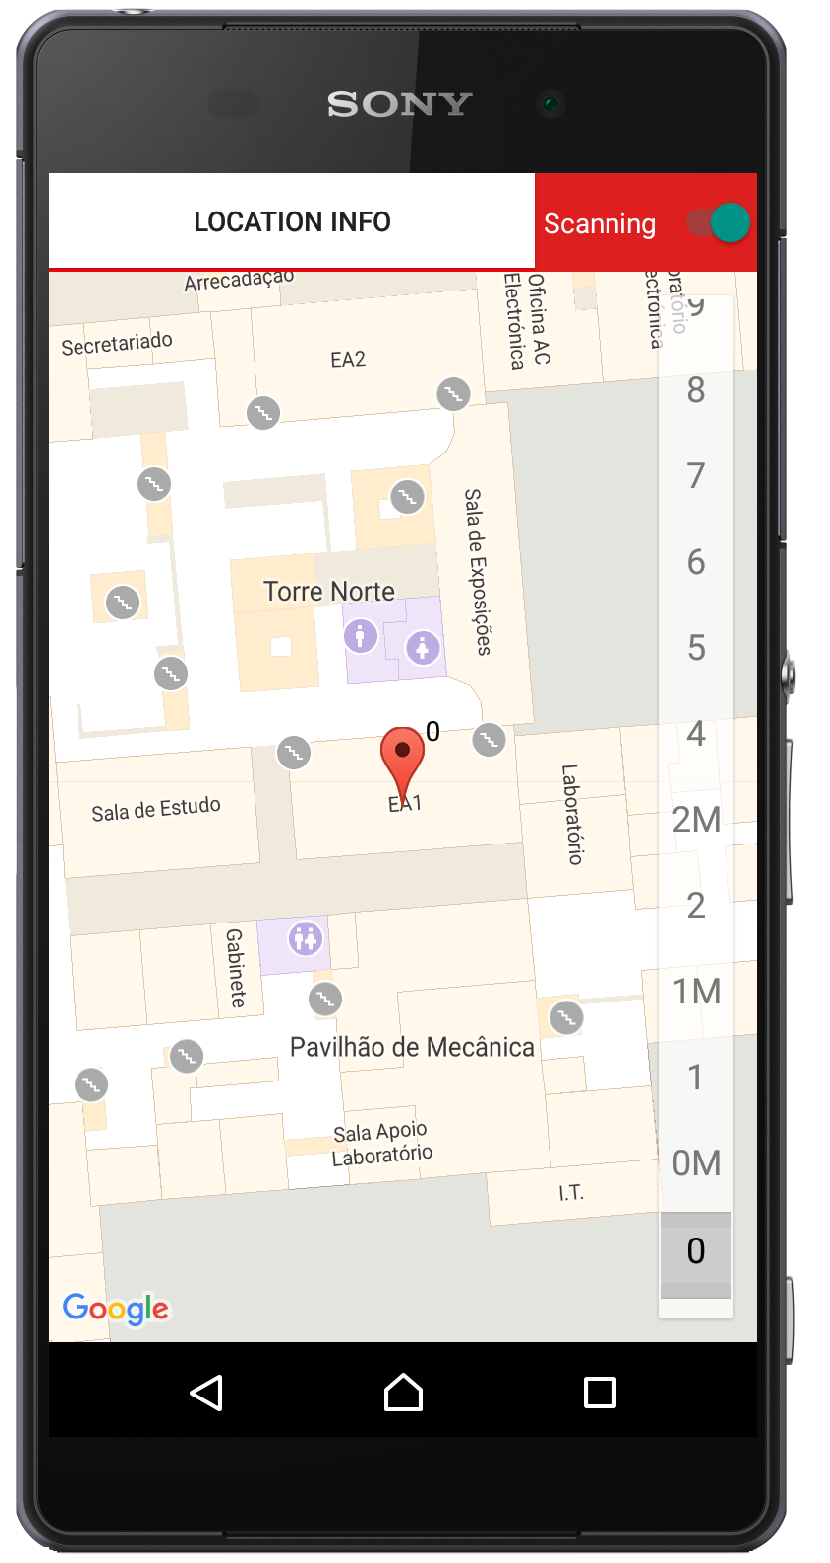
\includegraphics[width=0.5\linewidth]{4.Chapter/app_focused.png} 
\caption[Application screen showing a focused location on a room]{Application screen showing a focused location on a room} 
\label{fig:AppFocus} 
\end{figure} 
 
 
\begin{figure} 
\centering 
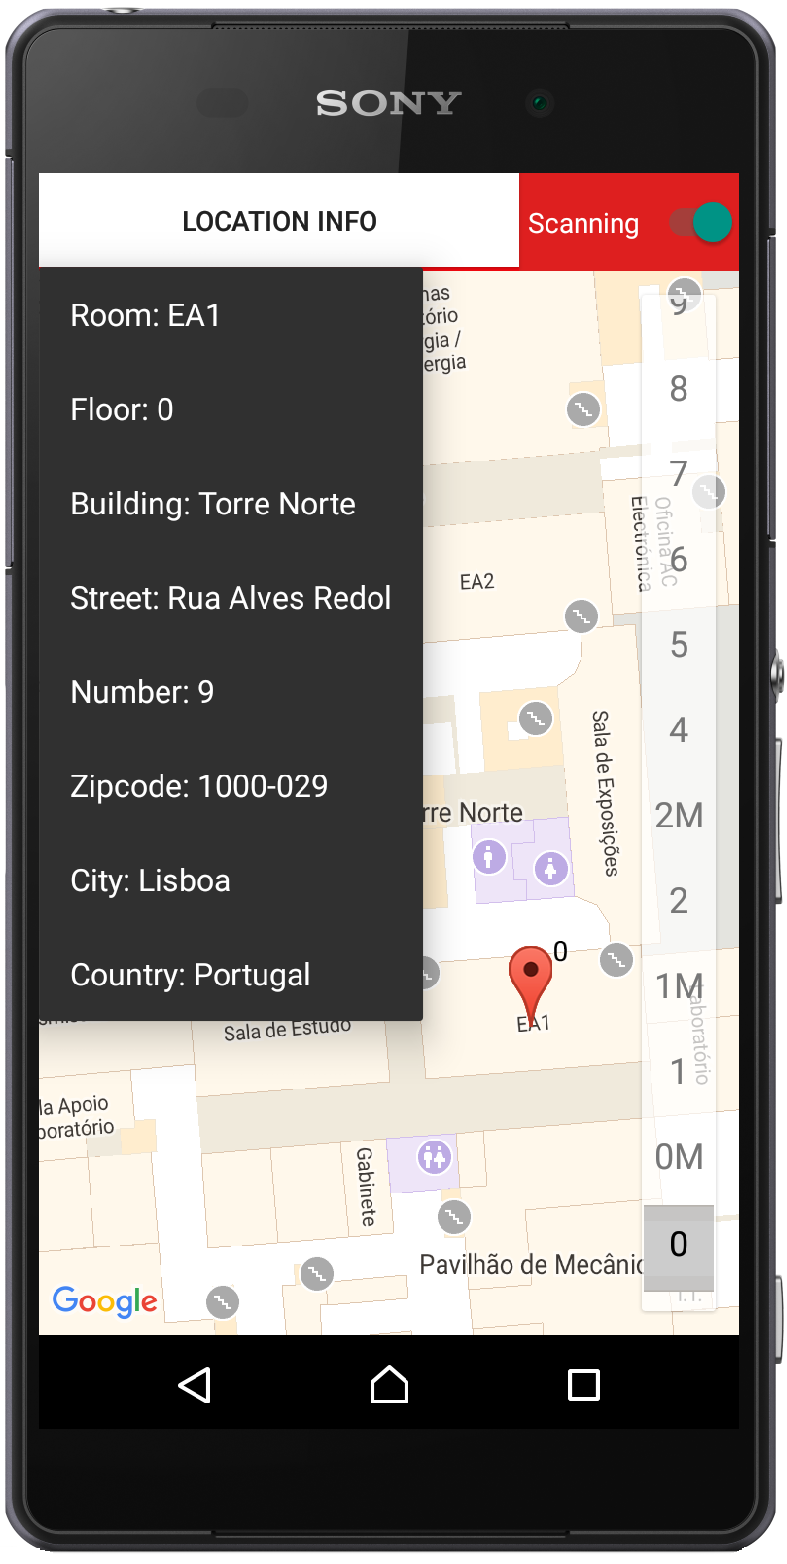
\includegraphics[width=0.5\linewidth]{4.Chapter/app_focused_menu.png} 
\caption[Application screen showing additional information of location]{Application screen showing additional information of location} 
\label{fig:AppMenu} 
\end{figure} 
 
 
 